\label{chap:basics}
This chapter represents the basic knowledge for the thesis work.
Section \ref{sec:memory_partition} introduces the memory
partitioning method with an existing formal power model.
Section \ref{sec:heuristics} discusses three potential
heuristics. In section \ref{sec:heuristics_selection}, the
discussed heuristics are compared with each other and the most
promising one is selected.
	\section{Memory partitioning and formal power model}
	\label{sec:memory_partition}
	This section is just a represent of the original work in the
	article \cite{Strobel2016} and no new material is included.
	
	There are two central concepts for memory power optimization
	using the memory partitioning method. One concept is the
	allocation $ \alpha $ which is a set of memory instances
	of certain memory types. The memory types are described
	by several parameters related to their physical
	characteristics.
	The other concept is the binding $ \beta $ of the application's
	code and data fragments to the selected memory instances.
	The code and data fragments of an application are referred
	as application profiles. And each application is represented
	by a set of profiles \cite{Strobel2016}. Every profile is
	characterized by some user-defined parameters.
	Table \ref{tab:memory_parameter} and Table
	\ref{tab:profile_parameter} describe the relevant parameters
	of the memory type and application profile respectively.
	Due to the fact that the memories are partitioned, an
	interconnect is included into the memory system. And this
	interconnect also requires power and area consumption.
	To take this factor into consideration for the memory power
	reduction, the interconnect is parameterized by its power and
	area consumption. Both parameters are related to the number of
	allocated memory instances. 
	
	\begin{table}[h]
		\begin{center}
			\small
			\begin{tabularx}{\textwidth}{|l|X|}
				\hline
				Parameter  		 & Description \\  \specialrule{1.2pt}{0pt}{0pt}
				Size			 & Provided memory space \\ \hline
				Area			 & Consumed on-chip area \\ \hline
				Read current 	 & Current required by the read operation \\ \hline
				Deselect current & Current required when no operation is performed \\ \hline
				Stand by current & Current consumed all the time \\ \hline
				Write current	 & Current required by the write operation (RAM only) \\ \hline
			\end{tabularx}
			\normalsize
			\caption{Memory Type Related Parameters}
			\label{tab:memory_parameter}
		\end{center}
	\end{table}

	\begin{table}[h]
		\begin{center}
			\small
			\begin{tabularx}{\textwidth}{|l|X|}
				\hline
				Parameter  		 	& Description \\  \specialrule{1.2pt}{0pt}{0pt}
				Duty cycle			& The active time frame in the profile's period\\ \hline
				Read probability	& The probability to perform the read operation in profile's duty cycle \\ \hline
				Write probability 	& Same with read probability except for write operation (RAM only) \\ \hline
				Size 				& Required memory space by the profile \\ \hline
			\end{tabularx}
			\normalsize
			\caption{Application Profile Related Parameters}
			\label{tab:profile_parameter}
		\end{center}
	\end{table}
	
	A configuration for the memory system is defined as a pair
	of an allocation of memory instances and the corresponding
	binding for the application profiles.
	Through the memory partitioning, an optimal configuration 
	is expected to be found such that the average power
	consumption by the selected memory instances is the lowest
	under certain predefined constrains. To achieve this
	optimization objective, a formal power model with four
	constraints are defined by the authors of \cite{Strobel2016}.
	In the following, some concepts related to the existing
	power model along with the constraints are introduced.
	
	Let $M$ denotes the memory type set used in the memory system.
	The allocation $\alpha$ is represented as a vector whose size
	is the number of memory types in the set, 
	$\alpha \in \mathbb{R}_{0}^{\lvert M \rvert}$.
	Each element in $\alpha$ is the number of instance for the
	corresponding memory type and its value should be
	non-negative.
	Let $A$ denotes the application set provided in the problem
	set.
	For each application, let $P_{a}$ represent its profile set.
	Then the binding $\beta$ to the corresponding $\alpha$
	is in the form of a binary matrix with size
	$ \arrowvert P_{a} \arrowvert \times \arrowvert M \arrowvert $,
	$ \beta \in \left\lbrace 0, 1 \right\rbrace
	^{\arrowvert P_{a} \arrowvert \times \arrowvert M \arrowvert} $.
	If the matrix element value $\beta_{aij}$ of an application $a$
	is 1, it means that the profile $i$ of application $a$ is bound
	to the memory type $j$. Otherwise, the memory type $j$ does not
	contain the profile $i$ for application $a$.
	
	The following are the four predefined constraints.
	
	\begin{itemize}
		\item Constraint 1 \\
			Define a fixed integer number $mems_{max}$, 
			The total number of the allocated memory instances
			should not exceed $mems_{max}$.
			\begin{equation}
			\label{equa:constraint_1}
				\sum_{i=1}^{\lvert M \rvert} \alpha_{i}
				\leq mems_{max}
			\end{equation}
		\item Constraint 2 \\
			Define a vector $A_{M}$ with size of $\lvert M \lvert$,
			$A_{M} \in \mathbb{R}^{\lvert M \lvert}$. Each element in
			$A_{M}$ indicates the area consumption of the corresponding
			memory type.
			Define a function $A_{F} \colon \mathbb{N}_{0}
			\rightarrow \mathbb{R}$. $A_{F}$ outputs the area consumed
			by the interconnect according to the total number of allocated
			memory instances.
			The area required by both memory instances and the interconnect
			should be limited to a maximum value, $area_{max}$.
			\begin{equation}
			\label{equa:constraint_2}
				\sum_{i=1}^{\lvert M \rvert} \alpha_{i} \cdot A_{M,i}
				+ A_{F} ( \sum_{i=1}^{\lvert M \rvert} \alpha_{i} ) 
				\leq area_{max}
			\end{equation}			
		\item Constraint 3 \\
			For each application, every profile should be contained in one
			and only one memory type. If there are multiple applications, all
			of them should satisfy this constraint.
			\begin{equation}
			\label{equa:constraint_3}
				\forall a \in \left[ 1, \lvert A \rvert \right], 
				\forall i \in \left[ 1, \lvert P_a \rvert \right] \colon
				\sum_{j=1}^{\lvert M \rvert} \beta_{aij} = 1
			\end{equation}		
		\item Constraint 4 \\
			Define a vector
			$\sigma^{P_{a}} \in \mathbb{N}_{0}^{\lvert P_{a} \rvert} $
			whose elements indicate the memory consumed by the profiles
			individually.
			Define another vector
			$\sigma^{M} \in \mathbb{N}_{0}^{\lvert M \rvert}$
			where the total memory spaces of the memories types are
			recorded in the corresponding elements.
			For every application, each memory type should have large enough 
			memory space to contain all the profiles that are bound to it.
			\begin{equation}
			\label{equa:constraint_4}
				\forall a \in \left[ 1, \lvert A \rvert \right], 
				\forall j \in \left[ 1, \lvert M \rvert \right] \colon
				\sum_{i=1}^{\lvert P_{a} \rvert} \beta_{aij} \cdot
				\sigma_{i}^{P_{a}} \leq \alpha_{j} \cdot \sigma_{j}^{M}
			\end{equation}
	\end{itemize}

	The configurations satisfy all the introduced constraints are considered
	as valid for the optimization problem and their average power consumption
	is computed as following model. Here, the illustration for the power model
	is focused on ROM first where only read operations are required.
	\begin{equation}
	\label{equa:p_mem}
		P_{j}\left( a \right) =
		P_{read,j}\left( a \right) +
		P_{desel,j}\left( a \right) +
		P_{stdby,j}
	\end{equation}
	The power consumption of one single memory type is consisted of three parts.
	Let $P_{j} \left( a \right) $ denotes the power consumed by memory type $j$
	for the application $a$. Seen from Equation \ref{equa:p_mem}, the three power
	fractions are:
	\begin{description}
		\item[$P_{read,j} \left( a \right) $]
			, consumed power when reading from the memory.
		\item[$P_{desel,j} \left( a \right) $]
			, consumed power when the memory is deselected.
		\item[$P_{stdby,j}$]
			, power continuously consumed by the memory.
	\end{description}
	Equations \ref{equa:p_read} to \ref{equa:p_stdby} show how to compute
	the three power fractions individually. In these equations,
	$d_{i}$ and $p_{ri}$ are the duty cycle and read probability of application
	profile $i$ respectively.
	$I_{r,j}\left( f \right)$, $I_{d,j}\left( f \right)$ and $I_{s,j}$
	are the read, deselect and standby currents of memory type $j$ respectively.
	$V$ is the voltage of the power supply to the memory system.
	\begin{equation}
	\label{equa:p_read}
		P_{read,j}\left( a \right) = 
		\sum_{i=1}^{\lvert P_{a} \rvert} \beta_{aij}
		\cdot d_{i} \cdot p_{ri}
		\cdot I_{r,j}\left( f \right) \cdot V
	\end{equation}
			
	\begin{equation}
	\label{equa:p_desel}
		P_{desel,j}\left( a \right) =
		\left( \alpha_{j} - 
		\sum_{i=1}^{\lvert P_{a} \rvert} \beta_{aij}
		\cdot d_{i} \cdot p_{ri}
		\right)
		\cdot I_{d,j}\left( f \right) \cdot V
	\end{equation}

	\begin{equation}
	\label{equa:p_stdby}
		P_{stdby,j} =
		\alpha_{j} \cdot I_{s,j} \cdot V
	\end{equation}		

	In this model, $P_{j} \left( a \right) $ is regard as the unit power for
	calculate the total power consumed by all memories for all applications.
	The average power consumption $P_{avg}$, also includes the contribution
	of the interconnect. Let $P_{F}$ denotes the function that outputs the
	power required by the interconnect. Then,  $P_{avg}$ is computed
	according to Equation \ref{equa:p_avg}.
	\begin{equation}
	\label{equa:p_avg}
		P_{avg} = P_{F}(\sum_{i=1}^{\lvert M \rvert}\alpha_{i}) +
		\frac{1}{\lvert A \rvert}
		\sum_{a=1}^{\lvert A \rvert} \sum_{j=1}^{\lvert M \rvert}
		P_{j}\left( a \right) 
	\end{equation}						
	
	\section{Heuristics}
	\label{sec:heuristics}
	There are a lot of existing heuristics. At the early time of heuristics usage, the algorithms are applied to solve one
	particular optimization problem. These problem-dependent heuristics cannot be adapted to other optimization processes.
	To improve the portability of heuristics, some algorithms are invented as parameterized interface that can be widely
	deployed for a variety of optimization problems. Such problem-independent heuristics usually consist of a base framework
	with several parameters. Only the parameters are related to the optimization problems. When using one of those
	heuristics for different problem sets, the algorithm framework is common while the parameters should be set up according
	to the problem requirements. In the recent years, there is a new trend of heuristic which is called hyper-heuristic.
	The hyper-heuristics provide a high-level strategy to seek one or several low-level heuristics to generate a proper algorithm for solving an optimization problem. The hyper-heuristic is a cutting-edge technique and it is beyond the knowledge of this work. For the memory power optimization, the problem-independent heuristics are the mainly focused
	because of its extensive usage.
	
	There are a variety ways to classify the heuristics. One common classification is to differentiate the algorithms
	according to their searching mechanisms. To be simplified, the heuristics are divided as local search-based and
	non-local search-based in this work. The well known local search algorithm aims to seek for the optimal solution by
	iteratively moving to a better solution in the neighborhood. However, the local search is greedy and cannot guarantee providing the good enough solutions because it may trap in local optimums. The idea of local search-based heuristics
	is to avoid the local optimum trap through some criteria for solution selection and improve the result's quality.
	Heuristics of this kind output only one single optimal solution. Some classical local search-based heuristics are simulated annealing, tabu search, guided local search, etc. Unlike local search-based heuristics, the non-local search-based heuristics usually seek for a set of good enough solutions. By manipulating some defined solution characteristics, it can guide the searching process to the global optimums. Some typical non-local search-based heuristics are genetic algorithm, particle swarm optimization, ant colony optimization, etc.
	Normally, the frameworks of non-local search-based heuristics are more complicated than that of local search-based algorithms. And the expected result for memory power optimization is one optimal configuration not a set of
	configurations. Therefor, the local search-based heuristics are the main focuses in this work.
	In this section, the local search algorithm along with its local optimum trap is discussed first. Then, two typical
	local search-based heuristics, tabu search and simulated annealing, are represented. Lastly, the most promising algorithm 
	is proposed to the memory power optimization according to the comparison between these heuristics.
	
		\subsection{Local search algorithm}
		\label{subsec:local_search}
		Local search algorithm is one of the simplest heuristics. Given a optimization problem, it starts from an initial solution and searches in the current solution's neighborhood. If a better solution is found, the current solution is replaced by it. The searching process is repeated until there is no better solution in the current solution's neighborhood. Then it outputs the current solution as the algorithm result.
		
		\setlength{\textfloatsep}{0.2cm}
\begin{algorithm2e}[htb]
	\KwIn{an optimization problem}
	\KwOut{an optimal solution}
	current solution = initial solution\;
	\While{not terminate}
	{
		generate a neighboring solution\;
		evaluate the neighboring solution\;
		\If{neighboring solution is better than current solution}
		{
			current solution = neighboring solution\;
		}
	}
	\Return current solution\;
	\caption{Local Search Algorithm}
	\label{algo:local_search}
\end{algorithm2e}
\setlength{\textfloatsep}{0.2cm}
		
		Algorithm \ref{algo:local_search} shows the pseudo-code of local search process. There are four main steps in the algorithm. First step is finding a initial solution and set it as the current solution. The initial solution should be valid for the problem. In the second step, a neighboring solution is generated by certain mechanism. And the third step is to compare the neighboring solution with the current one through a object function. The object function is a method to indicate how good the solution is. The last step is the selection criterion for solution. Local search algorithm selects the better one between the current and neighboring solutions, which is a naive criterion.
		
			\begin{figure}[H]
				\begin{center}
					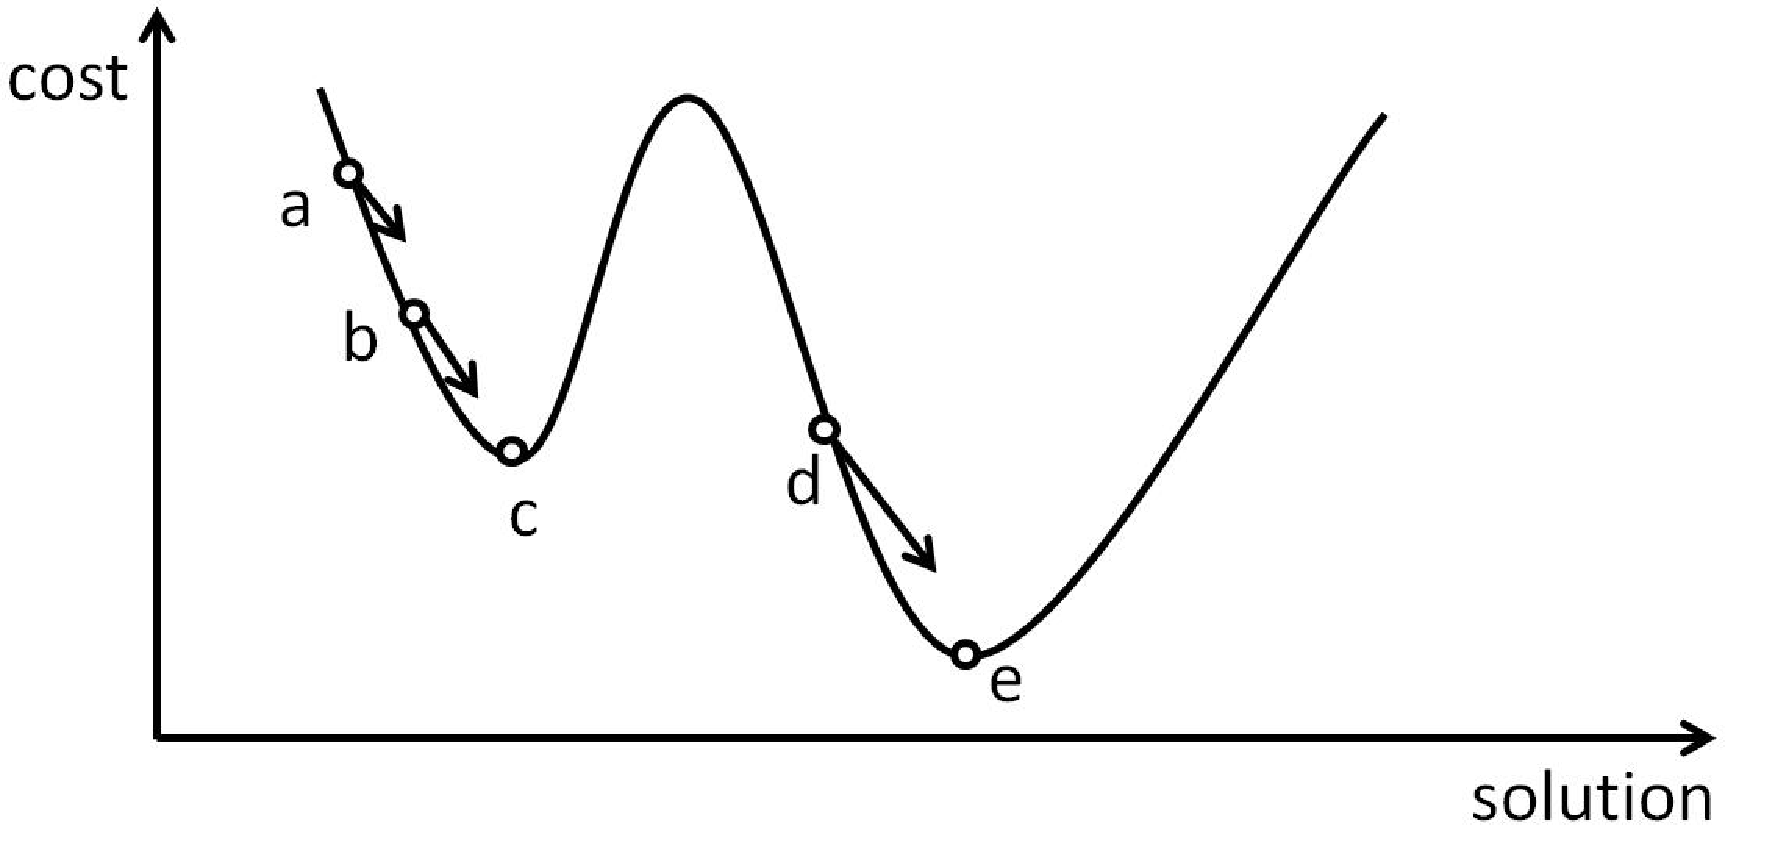
\includegraphics[width=0.7\textwidth]{local_optimum_local_search}
					\caption[Local Optimum Trap]{Local Optimum Trap}
					\label{fig:local_optimum_local_search}
				\end{center}
			\end{figure}
		
		Though local search algorithm is simple, the solution it provides may be the local optimal one. This is the major problem of
		local search algorithm. Figure \ref{fig:local_optimum_local_search} illustrates this local optimum trap. Suppose the
		optimization problem is to find the solution with minimum cost, the local search algorithm starts with the initial solution $a$.
		The cost of neighboring solution $b$ is lower than cost of $a$, then $b$ becomes the current solution. The same searching process 
		is repeated until the current solution reaches $c$. There is no better solution in $c$'s neighborhood, thus the algorithm outputs solution $c$ and terminates. However, solution $c$ is only the local optimum and the global optimum is solution $e$ which
		is not in $c$'s neighborhood. In order to reach solution $e$, the algorithm has to move to solution $d$ whose cost is higher than
		$c$'s cost. And this violates the selection criterion of the algorithm. Another drawback of local search algorithm is that the result quality is dependent on the initial solution. If the algorithm starts with solution $d$, the output will be the global optimum $e$. These two disadvantages make local search algorithm an improper choice when global optimal solution is required for 
		the optimization problems.
				
		\subsection{Tabu search algorithm}
		\label{subsec:tabu_search}
		One of the improvements to local search is the tabu search algorithm. It is based on local search but it avoids to stuck at the
		local optimal trap through a different selection strategy for solutions. As discussed in section \ref{subsec:local_search}, once
		the local search algorithm is trapped at a local optimal solution, it cannot move any further due to the naive solution criterion.
		To solve this problem, Fred Glover proposed the concepts of tabu list and the aspiration criterion in \cite{doi:10.1287/ijoc.1.3.190} and \cite{doi:10.1287/ijoc.2.1.4}.
		
		The key element of tabu search is the tabu list. It imitates the memory function of human brain to guide the searching process.
		It is used to record the tabu objects. The tabu objects can be defined as the solutions, solution movements or values of the 
		object function. Tabu list has a limited size which is one of the algorithm parameters. The improvement to local search algorithm
		is gained from the solution selection strategy that is usually called the tabu move. There are two rules in the tabu move. The
		first rule is to exclude the solutions recorded in the tabu list from a set of neighboring solutions. The second rule is to
		select the best in the rest of the neighboring solution set. The solution chosen by the tabu move is set as the current solution.
		Another concept of tabu search algorithm is the aspiration criterion. During the searching process, the best-so-far solution is
		kept recorded in the searching history. The aspiration criterion is to examine the neighboring solution set to find if there are solutions that are better than current best-so-far solution. If such solutions are found, then the best of them is selected and
		set as the current solution even if it is recorded in the tabu list. If no such solutions is found, the algorithm continues with
		the tabu move.
		
		\setlength{\textfloatsep}{0.2cm}
\begin{algorithm2e}[htb]
	\KwIn{an optimization problem, algorithm parameters}
	\KwOut{an optimal solution}
	set algorithm parameters\;
	current solution = initial solution\;
	best-so-far solution = initial solution\;
	set tabu list as empty\;
	\While{not terminate}
	{
		generate a set of neighboring solutions\;
		evaluate neighboring solutions\;
		\eIf{aspiration criterion satisfied}
		{
			execute aspiration criterion\;
			update current solution\;
			update tabu list\;
			update best-so-far solution\;
		}
		{
			execute tabu move\;
			update current solution\;
			update tabu list\;
		}
	}
	output current solution\;
	\caption{Tabu Search Algorithm}
	\label{algo:tabu_search}
\end{algorithm2e}
\setlength{\floatsep}{0.2cm}		
		
		Algorithm \ref{algo:tabu_search} is the pseudo-code of tabu search framework based on the Fred Glover's proposal in \cite{doi:10.1287/ijoc.1.3.190}. 
		At the beginning of the algorithm, it generates a valid initial solution and set it as the current solution and the best-so-for solution. The parameters are set up according to the algorithm inputs. And a tabu list is created as empty.
		After the initialization, the algorithm generates a set of neighboring solutions by some certain mechanism and evaluate it by an object function. After this step, there are two different branches.
		One branch is the execution of aspiration criterion. If the condition of the criterion is satisfied, the solution selected by the
		criterion is set as the current solution and the best-so-far solution. Also, the updated current solution is added to the tabu
		list. There are two cases for the tabu list updating. At the early stage of the algorithm, the list is not full. The solutions are added into the list sequentially. When there is no space for a new recorded solution, the oldest solution in the list is replaced by the new one.
		The other branch, tabu move, is executed when the condition of aspiration criterion is not satisfied. The current solution and the tabu list are updated with the solution chosen by the tabu move. And the best-so-far solution is not updated because there is no solutions better than it.
		The same searching process is repeated until the termination condition is satisfied and the algorithm outputs the current or the best-so-far solution as the optimization result. Some algorithm parameters are related to the termination condition. One simple
		method to terminate the algorithm is to set a fixed iteration number. Thus this fixed number is one parameter of the algorithm. However, this method cannot guarantee the solution quality. Another common termination mechanism is to count the appearance of the current solution. If the current solution dose not change for a max number iterations, the algorithm can terminate. Therefor,
		this max number is also one algorithm parameter.

		\begin{figure}[H]
			\begin{center}
				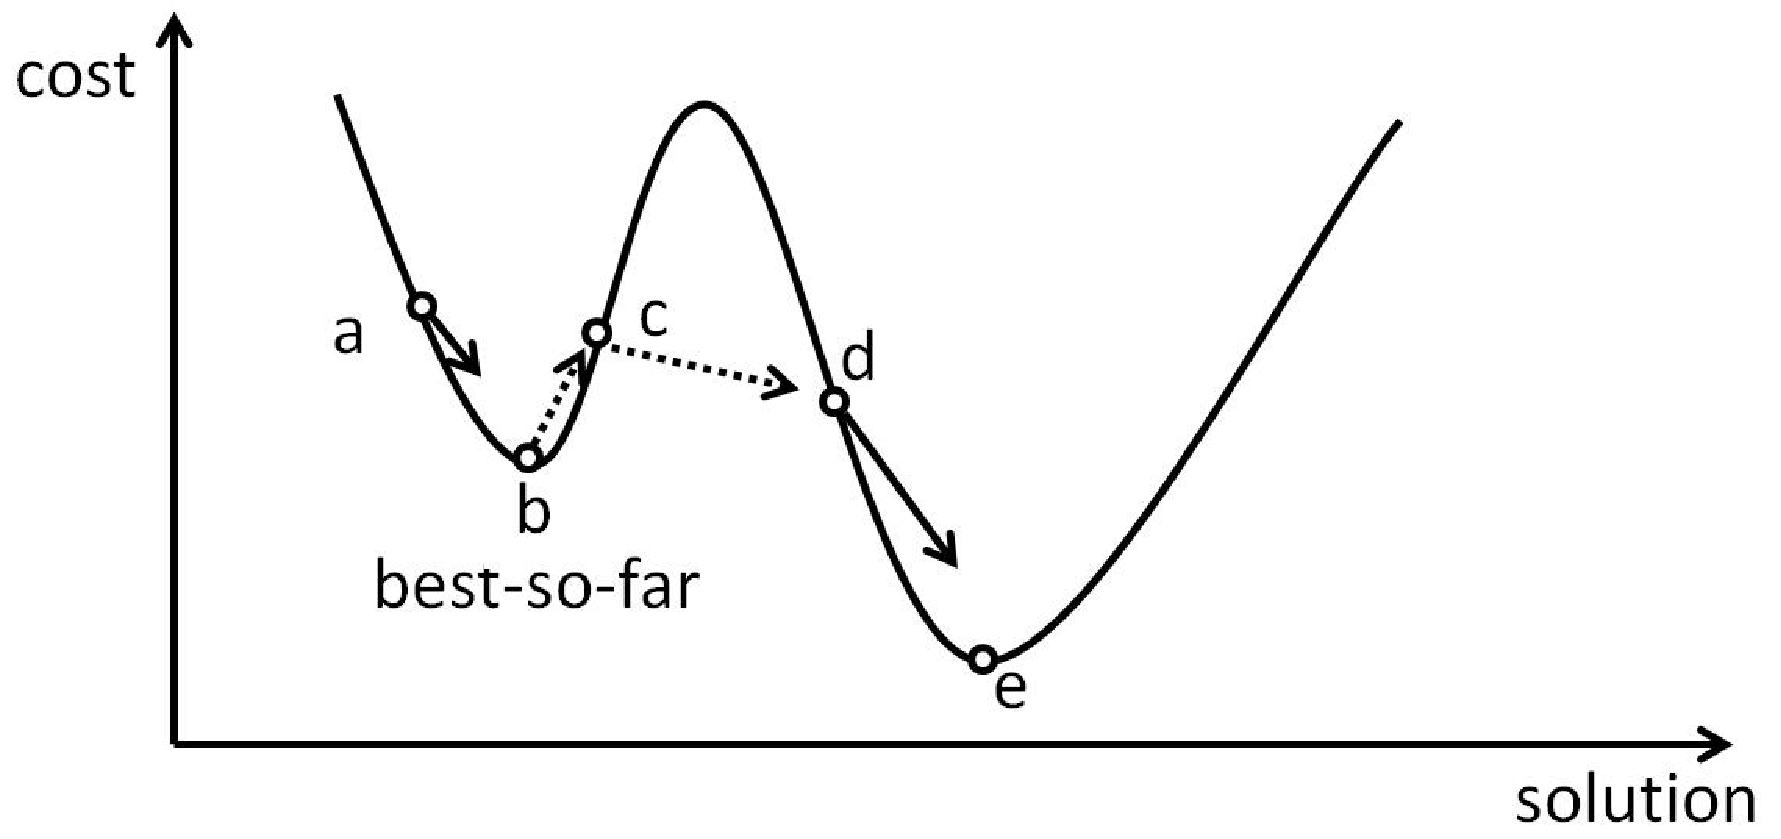
\includegraphics[width=0.7\textwidth]{local_optimum_tabu}
				\caption[Tabu Search's Avoidance to Local Optimum Trap]{Tabu Search's Avoidance to Local Optimum Trap}
				\label{fig:local_optimum_tabu}
			\end{center}
		\end{figure}

		
		Figure \ref{fig:local_optimum_tabu} illustrates how the tabu search algorithm avoids the local optimum trap. The solid line represents the execution of the aspiration criterion and the dotted line is the tabu move.
		The same problem set in section \ref{subsec:local_search} is used. The tabu search algorithm starts from initial solution $a$ with an empty tabu list (assume the list size is large enough).
		After the neighboring solutions are generated, it finds solution $b$ satisfies the aspiration criterion. Then $b$ becomes the current
		solution and the best-so-far solution is updated to $b$ as well. Also, $b$ is added to the tabu list. Known from the figure, solution $b$ is
		a local optimum and there is no neighboring solution satisfies the aspiration criterion. Thus, the algorithm continues with the tabu move.
		During the tabu move, solution $b$ is excluded from the generated neighboring solution set because it is stored in the tabu list.
		And solution $c$ is found to be the best among the rests of the set. Thus, $c$ becomes the current solution and it is added to the tabu list.
		In the next iteration, solution $b$ and $d$ both are $c$'s neighboring solutions. However, $b$ is still in the tabu list and the aspiration
		criterion is not satisfied. Thus, the current solution $d$ is selected by the tabu move as it is the best among the rest of neighboring solutions.
		The same searching process is repeated until the algorithm reaches solution $e$ which is the global optimum.
		By selecting a worser solution in the tabu move, the tabu search algorithm can move to a new searching region and avoid the local optimum trap.
	
		\subsection{Simulated annealing algorithm}
		\label{subsec:simulated_annealing}
		An other enhancement for the local search is the simulated annealing algorithm.
		The idea of the algorithm is to imitates the metal annealing process. Three steps
		are performed in the annealing process. First, the metal is melted at a very high
		temperature. The second step is to wait until the metal reaches its equilibrium
		state at the current temperature level. Then in the third step, the metal is
		cooled down slowly. The last two steps are repeated until the normal temperature
		is reached and the metal is in the ground state. Inspired by this process, the
		simulated annealing algorithm is proposed in \cite{10.2307/1690046}. And in the
		algorithm, the metropolis criterion is introduced to avoid the local optimum trap.
		
		The metropolis criterion is a probabilistic technique to choose the solutions.
		In the local search algorithm, the better neighboring solutions are always selected
		and it is not possible to accept a worser one. In the simulated annealing
		algorithm, the metropolis criterion accepts the neighboring solution with a 
		probability which is related to a control parameter. The control parameter
		is the imitation of the temperature in the metal annealing precess.
	
		\begin{equation}
		\label{equa:metropolis_equation}
			p=
				\begin{cases}
					1 & \text{, if } s_{next} \text{ is better than } s_{current}\\
					\exp{\left( -\frac{f(s_{next})-f(s_{current})}{t} \right)} & \text{, otherwise}\\
				\end{cases}
		\end{equation}
		
		Equation \ref{equa:metropolis_equation} represents the computation of the accept
		probability. In the equation, $s_{next}$ is the next neighboring solution of the
		current solution $s_{current}$. $p$ is the probability to accept $s_{next}$.
		And $f()$ is the object function. The value of $f()$ is referred as the
		solution cost. $t$ is the control parameter. It is can be seen from the equation
		that if $s_{next}$ is better than $s_{current}$, the metropolis criterion behaves
		like the local search algorithm. And if $s_{next}$ is worser, it can still be accepted
		depend on the computed probability. One thing is noticed in \cite{10.2307/1690046}
		is that the difference between costs of $s_{next}$ and $s_{current}$ should be a
		positive value. Thus in the second case of the equation, the accept probability
		becomes smaller with the decrease of the control parameter's value.
		
		The basic idea of simulated annealing algorithm is to combine the local search
		with the imitation of metal annealing process. And the metropolis criterion is
		used to improve the solution quality.
		The algorithm searches better solution in current solution's neighborhood at 
		different temperature levels.
		The searching process at the same temperature is repeated until certain termination
		condition is satisfied. The temperature is controlled to be reduced step by step
		as the same cooling procedure executed in metal annealing process. At the early
		stage of the algorithm, the current solution is updated randomly because a lot of
		worser solutions are accepted due to the high temperature. However, with
		the decrease of the temperature, the probability to select worser solution becomes
		smaller. This makes the searching space closer to the optimal region.
		
		\label{chap:simulated_annealing}
This chapter introduces the simulated annealing.
		
		Algorithm \ref{algo:simulated_annealing} shows the pseudo-code of the simulated
		annealing process. In the preparing stage, the algorithm sets up the parameters
		according to the algorithm inputs. And the initial solution is set as the current
		solution. The temperature $t$ is set up to a high enough value so that the random
		solutions can be selected by the metropolis criterion.The main framework of the
		simulated annealing can be divided into two nested loops. The outer loop is just the
		reduction of the temperature.
		The inner loop is the execution of local search with metropolis criterion.
		Firstly, the neighboring solution is generated by certain mechanism and evaluated by the
		object function. Then the current solution is updated according to the result from
		the metropolis criterion.
		The inner and outer loop terminate when some predefined conditions are satisfied.

		Figure \ref{fig:local_optimum_sa} illustrates how the simulated annealing algorithm
		can avoid the local optimum trap. The solid line represents the acceptance of better
		solution while the dotted line is the acceptance of worser solution.
		The same problem of \ref{subsec:local_search} is used.
		Suppose the current solution is $a$ at a proper temperature level. The algorithm finds
		the neighboring solution $b$ is better. Through the metropolis criterion, the current
		solution is updated to $b$ which is the local optimum. In the following iteration, the 
		neighboring solution $c$ with higher cost is generated. Because of the proper
		temperature, it is possible to accept $c$ with the computation of the accept probability.
		And the same searching process is repeated until the global optimal solution $e$ is reached.
		It is still possible that the algorithm moves away from $e$ at current temperature.
		However, the current temperature is assumed to be proper. And it applies that even if the
		global solution $e$ is discarded by the metropolis criterion, the selected solution can not
		be much worser than $e$. If the algorithm terminates at this current temperature, a near
		optimal solution can be obtained. And if the algorithm continues with the decrease of
		the temperature and a low enough temperature is reached, it can move back to $e$ agian
		and a worser solution can not be selected.
		 
		\begin{figure}[H]
			\begin{center}
				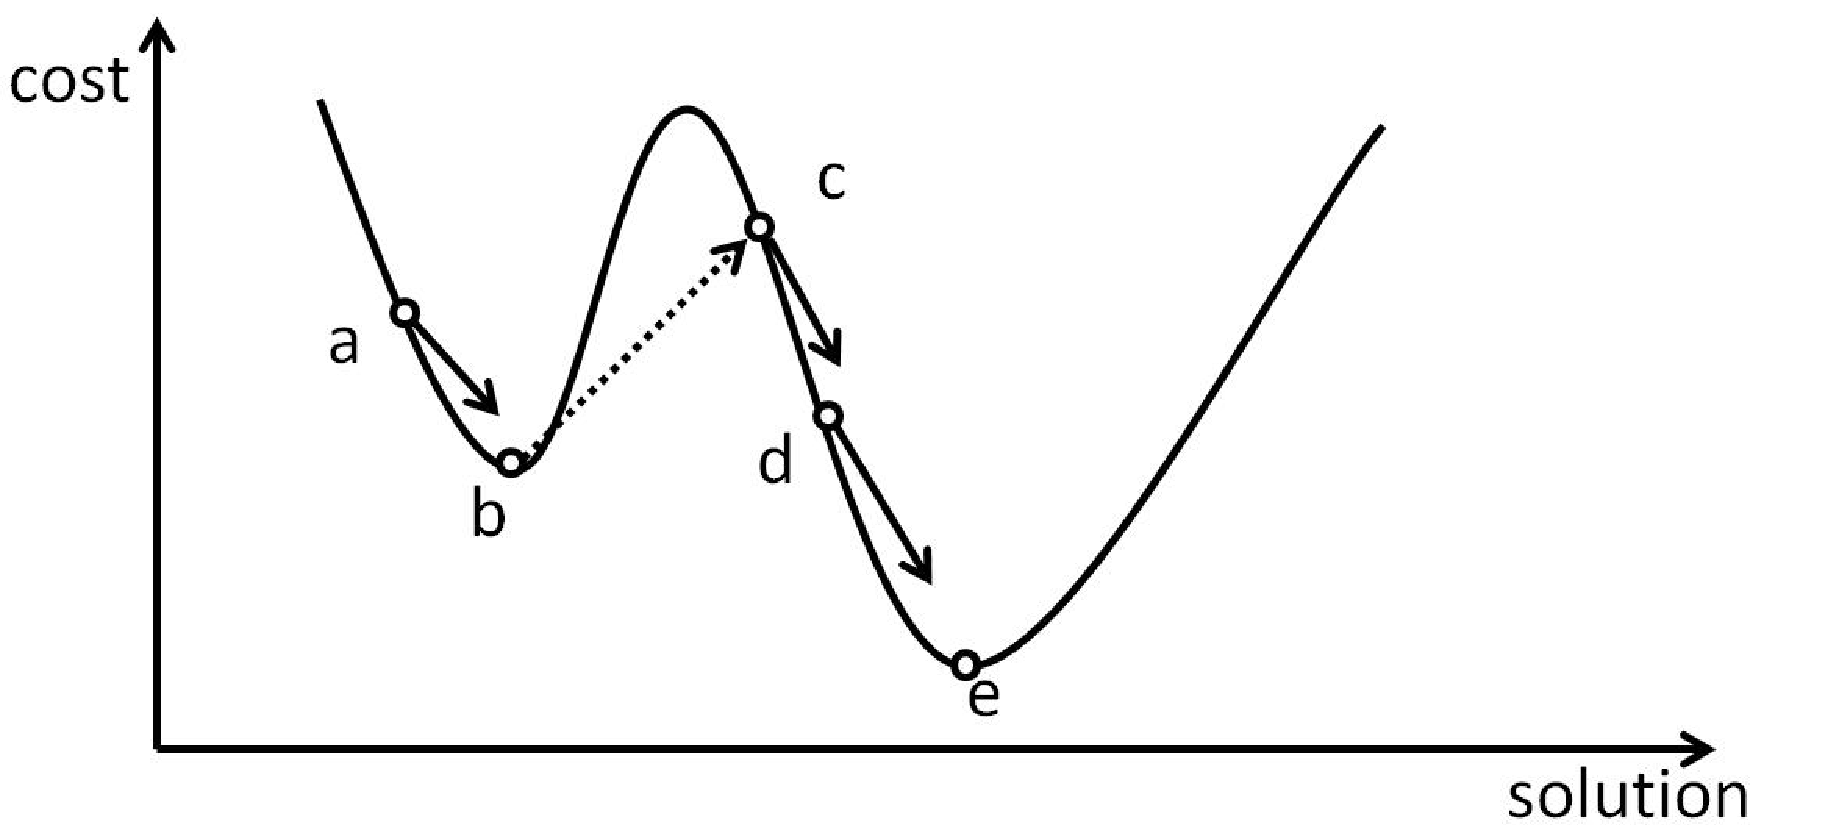
\includegraphics[width=0.7\textwidth]{local_optimum_sa}
				\caption{Simulated Annealing's Avoidance to Local Optimum Trap}
				\label{fig:local_optimum_sa}
			\end{center}
		\end{figure}
		
	\section{Heuristics selection}
	\label{sec:heuristics_selection}
	Though the discussed heuristics in Section \ref{sec:heuristics} seem to
	be the potential approaches for the memory power optimization problem.
	However, each of them has its own advantages and disadvantages.
	
	The local search algorithm is simple and it can be easily adapted to the
	optimization process. But it can not guarantee the solution quality
	even for the near optimal one because of the local optimum trap. Thus,
	the local search algorithm is not taken into consideration according
	to the optimization goal.
	
	The tabu search algorithm uses the tabu list as the memory structure to
	guide the searching process. By forbidden the recorded solutions, it can
	exclude the previously searched space to avoid the search repetition.
	As discussed in Section \ref{subsec:tabu_search}, once the algorithm
	traps in the local optimum, worser solutions can be selected by the
	tabu move. And the aspiration criterion helps the algorithm move to the new
	searching spaces.
	However, the tabu list size is the essential parameter
	and it can affect the algorithm performance. If the list size is too
	small, the algorithm may be trapped in a searching loop. In this case,
	the algorithm will stick to the local optimum trap. Because of the small
	tabu list size, the local optimal solution is recorded for a short
	period and it is released before the algorithm can move to a better
	searching space. If the list size is too large, the searching time will
	be quite long and it may be not acceptable in practice. Besides the tabu
	list size, the algorithm performance is also dependent on the initial
	solution. And selecting a proper initial solution is a non-trivial work.	
	Another drawback of tabu search algorithm is the dead lock problem.
	In some extreme cases, there is no solution satisfies the aspiration
	criterion in the current solution's neighborhood. And all the neighboring
	solutions are recorded in the tabu list. Then no solution will be selected
	and the algorithm can not continue.
	
	As discussed in Section \ref{subsec:simulated_annealing}, the simulated
	annealing algorithm can deal with the local optimum trap properly.
	And it is not sensitive to the initial solution. Because at the early
	stage of the algorithm, the metropolis criterion selects the solution
	randomly due to the high temperature. Even if the initial solution is
	already good enough, the algorithm may move far away from it. With the
	slow decrease of the temperature, the algorithm moves to optimal searching
	region step by step.
	Nevertheless, the initial temperature is one significant parameter of the
	simulated annealing. It is supposed to be high enough to make the metropolis
	criterion accepts solutions randomly. If it is too low, the algorithm
	behaves similarly to the local search and may be trapped in local optimum.
	If it is too high, an amount of time is wasted for the random searches.
	Another factor affects the solution quality of the simulated annealing is the
	cooling schedule. If temperature decreases too fast, the behavior of the local
	search occurs much earlier before the global optimal region is reached.
	If it decreases too slowly, the searching time will be quite long.
	Also, the termination conditions related to the nested loops play an important
	role in the simulated annealing algorithm. If the inner loop terminates too
	soon, the searching space is not fully explored. And if the outer loop ends too
	early, the accept probability is rather high. The final solution may be not
	good enough. If both loops terminate too late, the algorithm may not be efficient
	enough for the optimization problem.
	
	Compared with the tabu search algorithm, there are more parameters should be set
	carefully in the simulated annealing. But there is a variety of existing mechanisms
	to adjust them properly. Finding a suitable initial solution for the tabu search
	will increase the complexity of the optimization process.
	And it may require the pre-analysis of the solution space. Furthermore, the
	dead lock problem of the tabu search may result in the algorithm failure,
	which is risky for the users of the algorithm. After taking all the
	aspects into consideration, the simulated annealing algorithm is more
	promising than the tabu search algorithm. And it is proposed for the memory
	power optimization problem. At this stage, the fist goal of this thesis work
	is achieved.
	
	
	\begin{table}[h]
	\begin{center}
		\small
		\begin{tabularx}{\textwidth}{@{}l *3{>{\centering\arraybackslash}X}@{}}
			\hline
			Parameter  		 					& Local search 	& Tabu search 		& Simulated annealing	\\ \hline
			Avoidance to local optimum trap 	& No			& Yes				& Yes					\\ \hline
			Initial solution sensibility 		& Yes			& Yes				& No 					\\ \hline
			Essential parameters 				& -				& Tabu list size	& Initial temperature, cooling schedule \\ \hline
			Algorithm Termination 				& 1 loop		& 1 loop			& 2 nested loops \\ \hline
			Other problems 						& Provide random results & Dead lock &long search time  \\ \hline
		\end{tabularx}
		\normalsize
		\caption{Heuristics Comparison}
		\label{tab:heuristic_comparison }
	\end{center}
\end{table}	
	
	